%harihiom
\documentclass{llncs}

\usepackage[english]{babel}
%\usepackage[utf8]{inputenc}
%\usepackage{amsmath}
\usepackage{graphicx}
\usepackage{float}
%\usepackage{wrapfig}
%\usepackage{titlepic}
%\usepackage[colorinlistoftodos]{todonotes}
\usepackage{graphicx,epstopdf}
\usepackage{amsmath,amssymb,amsfonts,subfigure}
\usepackage{comment}
\usepackage{algorithm}
\usepackage{algpseudocode}
\usepackage{pifont}
\usepackage[normalem]{ulem}
\usepackage[english]{babel}
\usepackage[utf8x]{inputenc}
\usepackage{graphicx}
\usepackage{calc}
\usepackage{graphicx}
\usepackage{subfigure}
\usepackage{gensymb}
\usepackage{natbib}
\usepackage{url}
\usepackage[utf8x]{inputenc}
\usepackage{amsmath}
\usepackage{graphicx}
\graphicspath{{images/}}
\usepackage{parskip}
\usepackage{fancyhdr}
\usepackage{vmargin}
\usepackage{algorithm}
\linespread{1}
\usepackage{color}
\usepackage{cite}
\usepackage{amsmath,amssymb}
\newtheorem{claim1}{Claim}
\usepackage{algpseudocode}% http://ctan.org/pkg/algorithmicx
\usepackage[compatibility=false]{caption}% http://ctan.org/pkg/caption
\setmarginsrb{3 cm}{2.5 cm}{3 cm}{2.5 cm}{1 cm}{1.5 cm}{1 cm}{1.5 cm}

%\newtheorem{theorem}{Theorem}
%\newtheorem{lemma}{Lemma}

\title{Lecture - 1}
\author{Thursday, 28 July 2016 (15:20 - 16:10)}


\institute{Puzzles : Monty Hall Show, Coin Tossing Game}

\begin{document}
\maketitle
\section{The Monty Hall Show}

The Monty Hall problem is based on the American reality show - ``Let's make a deal'' and is named after its host, Monty Hall. \\

Before explaining the Monty Hall game, let us understand a simpler scenario. Assume you are the contestant of a reality show. On the stage, there are $3$ doors present in front of you. Out of these $3$ doors, $1$ door contains BMW car and rest of the two doors contain goats. You as a contestant do not know what is hidden inside these gates. You are asked to choose one gate and you get what is hidden inside the gate. Obviously, you are considered to win if and only if you choose the gate hiding the BMW car.  

In this simple scenario, probability of winning = $1/3$ and probability of losing = $2/3$.\\

\textbf{Now, we introduce the Monty Hall problem which brings in a twist to this simple scenario.}\\

Monty Hall is now the smart anchor of our show and enters the scene. He asks you to choose one door, similar to the previous case. You choose any one of the gates as in the previous case. But before declaring the result, Monty shows you the one gate hiding a goat out of the two gates which you have not chosen\footnote{Monty knows which door has what. That's why he is capable of opening a door which has a goat hidden.}. Since, there are two doors hiding goats, there is definitely atleast one goat in the gates which you have not chosen. Now, you are given an option to swap your choice and choose the third gate which is unopened and previously not chosen by you. This has been shown in Figure \ref{monty} \\

\begin{figure}[h]
\centering
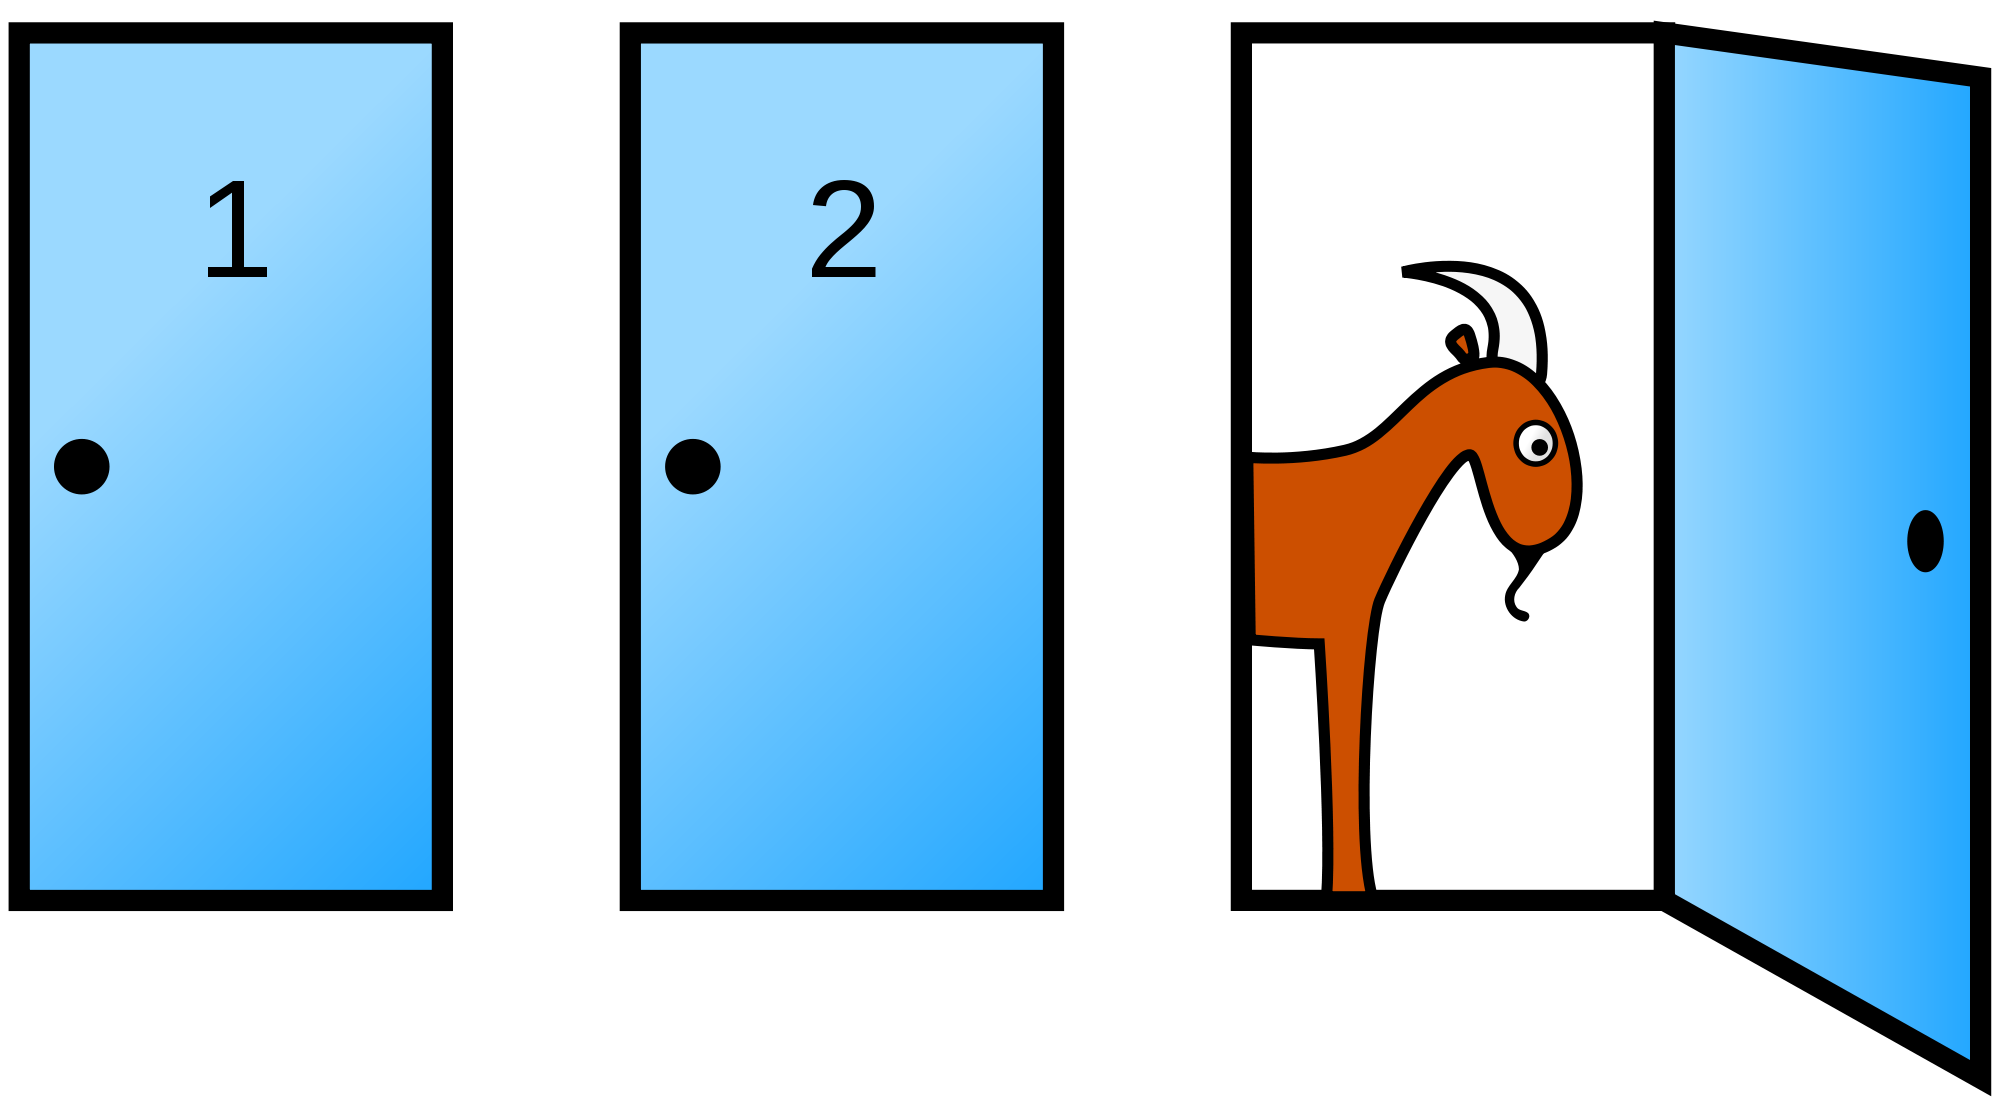
\includegraphics[width=0.5\textwidth]{monty.png}
\label{monty}
\caption{The Monty Hall Game}
\end{figure}

\textit{SHOULD YOU SWAP YOUR CHOICE AND GO WITH THIS THIRD GATE OR IT DOES NOT MATTER? Do you think swapping makes any difference to your probability of winning?}

Let us consider the two cases, one where you swap and the other where you do not swap. \\

\textbf{Case 1}:\textit{ You do not swap}: So, you have chosen one door and after knowing which of the other two doors has a goat, you do not swap your choice. So, this extra knowledge does not matter to your answer.
Hence, Probability (Win) = 1/3 and Probability (Losing) = 2/3

\textbf{Case 2:} \textit{You swap:}\\ 
\textit{Case 2.a :} You have initially chosen a door containing a goat.\\ 
Probability (You have chosen a door containing goat) = $2/3$. Now Monty shows you the other door having a goat. So, when you swap, you definitely pick the door having BMW. Hence, your probability of winning = $2/3$.\\

\textit{Case 2.b : }You have initially chosen the door containing BMW.\\ 
Probability (You have chosen the door containing BMW) = $1/3$. Now Monty shows you the other door having a goat. So, when you swap, you definitely pick the door having another goat. Hence, your probability of losing= $1/3$.\\

Hence, we see that swapping the gates results in the swapping of the probabilities of winning and losing thereby making win more likely. \\

\textbf{Hence, one must always swap the answer in such a scenario.} 

\textbf{Quick Brainteaser} : What is the probability of winning if participant tosses an unbiased coin to take this decision of swapping. If head comes, she swaps, else does not swap? \\
Answer:$1/2$ (Figure out how!)\\


\section{The Coin Tossing Game}
\textbf{The Game}: In a contest, a participant tosses a coin. If the coin shows up tail, an amount of $100$ \$ is placed on the table in front of him, and he continues tossing. If the coin shows up a head, an amount of $100$ \$ is kept on the same table and then all the money kept on the table is given to the participant concluding the game. It can be seen that the participant wins a cash amount of $100 \times number\ of\ coins\ tossed$. \\

\textbf{Question:} What is the expected value of cash price won by the participant?\\

\textbf{Answer}: 
Let $X$ be a random variable which counts the number of times the coin is tossed.\\

We know that $X$ can take the values 1, 2, 3, 4.......\\
$E[X]\ =\ 1 \times pr(X=1) + 2 \times pr(X=2) + 3 \times pr(X=3)+ .... $\\

= $\sum_{i=1}^{\infty} i \times pr(X=i) $\\

Since, $ pr(X=i) $ = $(1/2)^i$\\

Hence, $E[X]\ = \sum_{i=1}^{\infty} i/2^{n} $\\

= $1/2+(2/2^2)+(3/2^3)+(4/2^4)+.....\ =\ \alpha$, say\\

Now, $\alpha = 1/2+(2/2^2)+(3/2^3)+(4/2^4)+.....$ \hspace{5mm} ........(1)\\

$\alpha/2 = (2/2^2)+(3/2^3)+(4/2^4)+.....$\hspace{5mm} ........(2)\\

Subtracting equation (2) from equation (1) \\

$\alpha/2= (1/2)+(1/2^2)+(1/2^3)+.....$\\

It can be seen that the above expression is a geometric progression $a,ar,ar^2,ar^3......$, with $a=1$ and $r=1/2$.\\

We know that the sum of an infinite Geometric Progression = $\frac{a}{1-r}$ = $\frac{1/2}{1-1/2}$ (in this case) = $1$. \\

Hence, $\alpha/2\ = 1$\\

$\alpha=2$\\

$E[X]=2$\\  	\hspace{5mm} ........(3)

So, the expected amount of money won by the participant = $2 \times 100$ \$ = $200$ \$.\\

Now, we know that the expected amount of money won by the participant is $200$ \$. But, the standard deviation of the amount of money won (or the number of coin tosses done) can be very large\footnote{When the game is actually played, the participant can win $100$ \$ in one case, yet $500$ \$ in other case, yet $10000$ \$ in other case.}. Hence, it is important to look at the standard deviation of the random variable $X$, in addition to its expected value.\\

The formula for Standard Deviation, $\sigma(X)$, is given as :\\ 

$\sigma(X)$= $ \sqrt{(E[X- \mu])^2} $, where $\mu = E[X]$\\


= $ \sqrt{E[X^2 - 2 X \mu + \mu ^ 2]} $\\

= $ \sqrt{E[X^2 ]- 2 E[X] \mu + E[\mu ^ 2]} $\\

= $ \sqrt{E[X^2 ]- 2 \mu^2 + \mu ^ 2} $\\

= $ \sqrt{E[X^2 ]- \mu ^ 2} $\\

= $ \sqrt{E[X^2 ]- (E[X]) ^ 2} $\\

Hence, $\sigma(X)$=  $ \sqrt{E[X^2 ]- (E[X]) ^ 2} $	(4)\\

$X^2$ is also a random variable, which takes the values $1^2, 2^2, 3^2, 4^2..........$\\

$Pr(X^2=1^2) = Pr(X=1) = 1/2$\\

$Pr(X^2=2^2) = Pr(X=2) = 1/2^2$\\

... and so on \\

According the the expectation formula, $E[X^2] = 1^2 \times \frac{1}{2} + 2^2 \times \frac{1}{2^2} + 3^2 \times \frac{1}{2^3} + ............  $ = $\alpha$ say\\

$\alpha\ =\ \frac{1^2}{2^1} + \frac{2^2}{2^2} + \frac{3^2}{2^3} + \frac{4^2}{2^4} + .... $   \hspace{5mm} ........(5) \\	


$\alpha/2\ =\ \frac{1^2}{2^2} + \frac{2^2}{2^3} + \frac{3^2}{2^4} + \frac{4^2}{2^5} + .... $   \hspace{5mm} ........(6)  \\

Subtracting equation (6) from equation (5)\\

$\alpha/2\ =\ \frac{1^2}{2^1} + \frac{2^2-1^2}{2^2} + \frac{3^2-2^2}{2^3} + \frac{4^2-3^2}{2^4} + .... $    \\


or, $\alpha/2\ =\ \frac{1^2}{2^1} + \frac{(2+1)(2-1)}{2^2} + \frac{(3+2)(3-2)}{2^3} + \frac{(4+3)(4-3)}{2^4} + .... $    \\


or, $\alpha/2\ =\ \frac{1}{2^1} + \frac{3}{2^2} + \frac{5}{2^3} + \frac{7}{2^4} + .... $     \hspace{5mm} ........(7)\\	

Dividing equation (7) by equation (2)\\

 or, $\alpha/4\ =\ \frac{1}{2^2} + \frac{3}{2^3} + \frac{5}{2^4} + \frac{7}{2^5} + .... $  \hspace{5mm} ........(8)\\
 
 Subtracting equation (8) from equation (7)\\
 
$\alpha/4\ =\ \frac{1}{2} + \frac{2}{2^2} + \frac{2}{2^3} + \frac{2}{2^4} + .... $\\

or, $\alpha/4\ =\ 1 + \frac{1}{2^2} + \frac{1}{2^3} + \frac{1}{2^4} + .. $\\ 

or, $\alpha/4\ =\frac{3}{4}$, (applying the formula for sum of Geometric Progression)\\

$\alpha = 6$, \\

$E[X^2]=6$	\hspace{5mm} ........(9)\\

Substituting equation (3) and equation (9) in equation (4), \\

$\sigma(X)$=  $ \sqrt{6- 2 ^ 2} $\\

= $\sqrt{2}$\\

	
\textbf{Brain Teasers}
\begin{enumerate}
\item State whether series is convergent $\sum_{n=1}^{\infty} n/2^{n} $
\item State whether the series is convergent $\sum_{n=1}^{\infty} 1/n$ 
\end{enumerate}


\end{document}
